\documentclass[12pt, letterpaper]{article}
\usepackage{hyperref}
\usepackage{graphicx}
\usepackage[margin=1in]{geometry}

\title{Mini Game Hub \\ Bash | Python | PyGame }
\author{Harshitha \\ Poorna Sai}
\date{Spring - 2026}
\hypersetup{
    colorlinks=true,
    linkcolor=blue,  
    urlcolor=blue,
}
\begin{document}
\maketitle
\tableofcontents
\newpage

\section{Introduction}
This is a multi-user game hub starts with \textbf{bash} authentication and game play with a graphical interface (\textbf{GUI}) followed by leaderboard and some matplotlib charts.

\section{Modules}
There are many Libraries which we used to build this project.

\subsection{Standard Libraries}
\begin{itemize}
    \item \textbf{os} - os is used to handle file paths and checking file existence
    \item \textbf{sys} - sys was used to access command line arguments
    \item \textbf{datetime} - datetime module is used to get exact date time at which game ends
    \item \textbf{csv} - csv module is used to read history.csv
    \item \textbf{subprocess} - subprocess module is to run bash script from Python
\end{itemize}

\subsection{External Libraries}
\begin{itemize}
    \item \textbf{pygame-ce} - pygame-ce module is used to build a graphical interface for the games. It handles rendering of game boards, mouse click animations and overall game play display
    \item \textbf{numpy} - numpy module is used to update display and checking win and draw conditions using numpy Functions
    \item \textbf{matplotlib} - matplotlib module is used to generate some graphs and their display using data stored in history.csv 
\end{itemize}

\section{Design and Architecture}
It is designed as a modular project having multiple components with separate structures. The major components are User-authentication, Game play, rendering game display and displaying statistics. 
Different responsibilities are clearly separated.

\subsection{Modular Design}
\begin{itemize}
    \item \texttt{main.sh} - handles secure user authentication including first time users, password hashing using sha256sum command 
    \item \texttt{base-game.py} - has base game class and util functions used in games and game.py
    \item \texttt{game.py} - controls game flow and transition between pages and buttons
    \item \texttt{games/} - directory contains individual games with their specific game board, logic and win conditions
    \item \texttt{leaderboard.sh} - prints sorted table based on wins, losses or wins/loss ratio using data in history.csv
\end{itemize}

\subsection{Architectural Decisions}
\subsubsection{Object oriented Game play}
Created a base game class to represent 2 player generic, turn based board game in \texttt{base\_game.py}. Each game inherits this base class and have their specific win conditions, draw conditions and rendering display.
Inheritance is used because it increases code re-usability.

\subsubsection{PyGame GUI}
A seperate PyGame graphical interface is used to avoid text based gameplay in terminal and to give better experience to the end user. PyGame helps in creating display, showing animations.

\subsubsection{Data storing}
users.tsv is used to store user data which includes username and hashed password, history.csv is used to store winner, loser, date-time, game and isdraw after completion of a game.
tsv and csv file formats are used because of their readability, simplicity and ease of processing data. Gave win/loss ratio= 9999 if losses= 0.

\subsubsection{Flexibility}
os.path.join is used to platform independent file handling. tr -d to avoid trail space errors.

\section{Features Implemented}
A list of features implemented in the project:

\subsection{User Authentication (main.sh)}
\begin{itemize}
    \item Password hashing using sha256sum.
    \item Ensuring password is strong enough. (minimum six characters with atleast 1 digit and an alphabet)
    \item Error messages are displayed in red color and success messages in green color.
    \item Ensuring Player1 and Player2 are different.
    \item Giving signup option for first time users.
    \item Centering of main headings for clean display.
\end{itemize}

\subsection{Game play (game.py)}
\begin{itemize}
    \item \textbf{Interactive Buttons} - Changing display with mouse click, creative hover effects with different RBG colors.
    \item \textbf{Back Button} - Added back button at every stage to get easy trasitions between pages.
    \item \textbf{Quit Button} - To exit gameplay.
    \item \textbf{Append History} - Appending history to history.csv after completion of a game.
    \item \textbf{Font} - Added impressive fonts to display buttons and player turn.
    \item \textbf{Background Images} - Added background images for every page instead of just filling rbg colors.
\end{itemize}

\subsection{Games}
\begin{itemize}
    \item \textbf{Win Condition} - Is implemented for every game with checking for draw cases.
    \item \textbf{Handle Click} - This method is implemented to change display after clicking game board.
    \item \textbf{Preview Effects} - Added preview effects in Connect4.
    \item \textbf{Suggestions} - Implemented valid moves method in Othello to suggest the player for easy gameplay.
    \item Displaying no valid moves for a player in Othello.
\end{itemize}

\subsection{Leaderboard and Matplotlib charts}
\begin{itemize}
    \item Allowed user to select sorting preference in leaderboard.
    \item Displayed statistics per game per user basis.
    \item Increased wins of both players by 0.5 in a draw case.
    \item Generated 2 bargraphs and 1 pie chart using data in history.csv.
    \item Allowed user to select play again, display statistics or quit option after completion of a game.
\end{itemize}

\section{Directory Structure}
\begin{verbatim}
mini-game-hub/
|-- main.sh
|-- game.py
|-- base_game.py
|-- leaderboard.sh
|-- requirements.txt
|-- .gitattributes
|-- games/
|   |-- tictactoe.py
|   |-- othello.py
|   `-- connect4.py
|-- assets/
|   |-- background_images/
|   |   |-- connect4_bg.png
|   |   |-- tictactoe_bg.png
|   |   |-- menu_bg1.png
|   |   |-- menu_bg2.png
|   |   `-- othello_bg.png
|   |-- fonts/
|   |   |-- Celinda.ttf
|   |   `-- Retro.ttf
|-- users.tsv
|-- history.csv
`-- README.md
\end{verbatim}

\section{Installation and Setup}
Note: We hope python 3.10 was already installed in the system.
\\
If pygame was installed and not pygamme-ce, Run the following commands in terminal: \\ \\
\texttt{pip uninstall pygame} \\ 
\texttt{pip install pygame-ce} \\ \\
To install dependencies, run following command: \\ \\
\texttt{pip install -r requirements.txt}

\section{Running and Interaction}
How to Run? Enter the following command in terminal, you will get into the game. \\
\texttt{bash main.sh} \\

\subsection{Running main.sh}
After running \texttt{bash main.sh}, you will have to signup if you are a first time user by clicking a special character as shown in figure \ref{fig:User_authentication}.
If you have already signed up before, you will have to login with your previous username and passsword. After both players have successfully logged in, you will automatically directed to a graphical PyGame interface.

\begin{figure}[h]
    \centering
    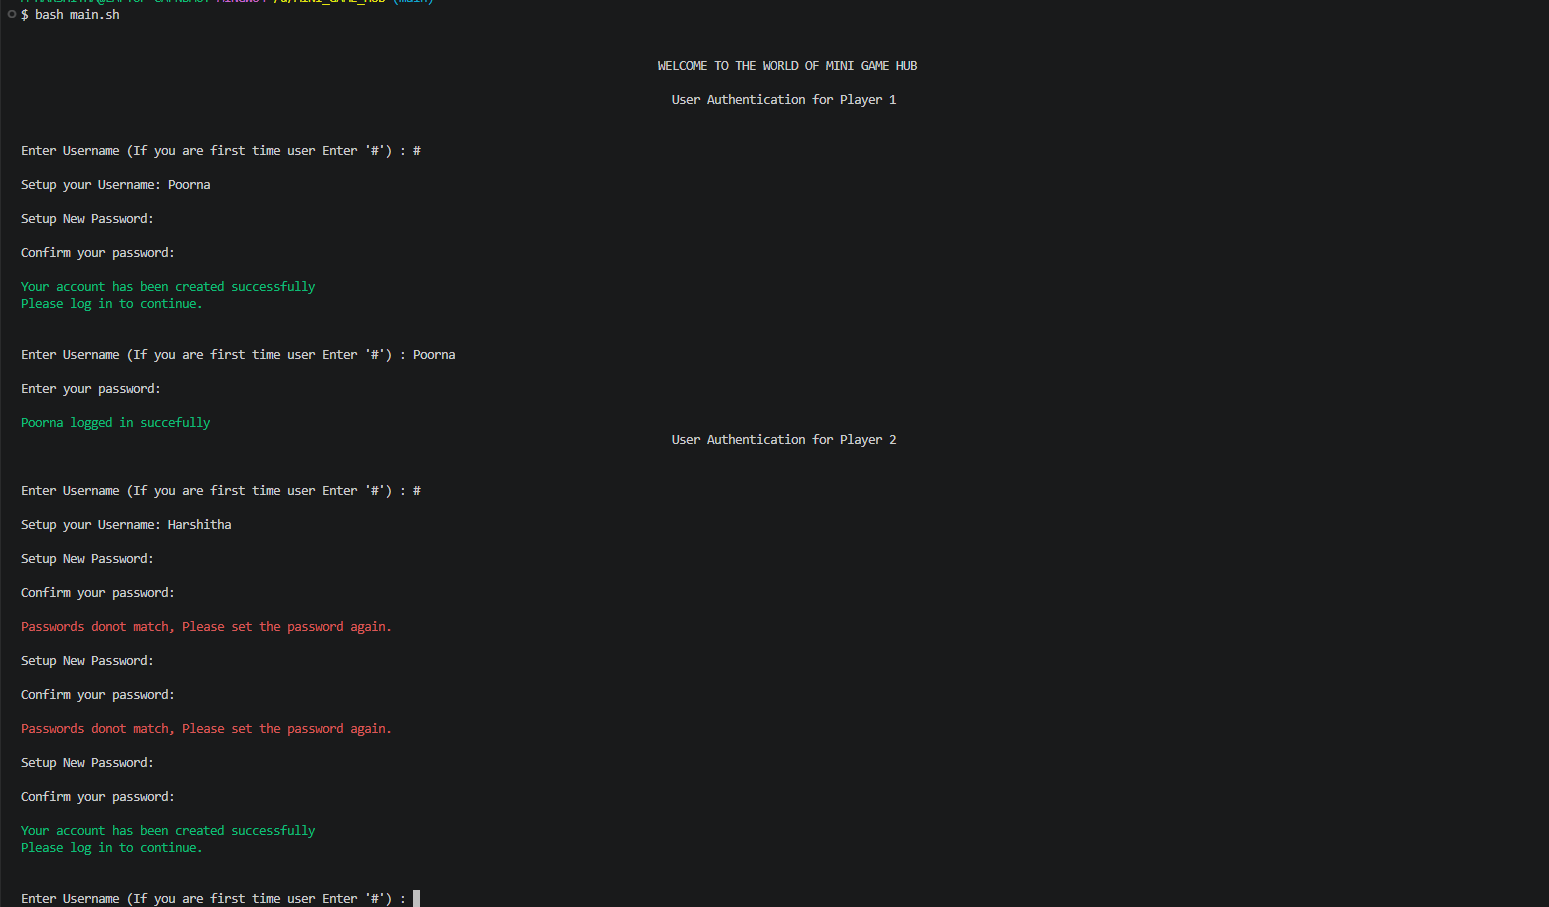
\includegraphics[width=1\textwidth]{User_authentication}
    \caption{User Authentication}
    \label{fig:User_authentication}
\end{figure}

\subsection{Interaction with GUI}
A PyGame GUI is displayed with Game menu and interactive Game buttons as shown in figures \ref{fig:PyGame1} and \ref{fig:PyGame2}. Back and Quit buttons are displayed which allows easier transtions for the users.
Hover effects are also added for better experience. You will be directed into the respective Game boards by clicking on the respective Game buttons.

\begin{figure}[h]
    \centering
    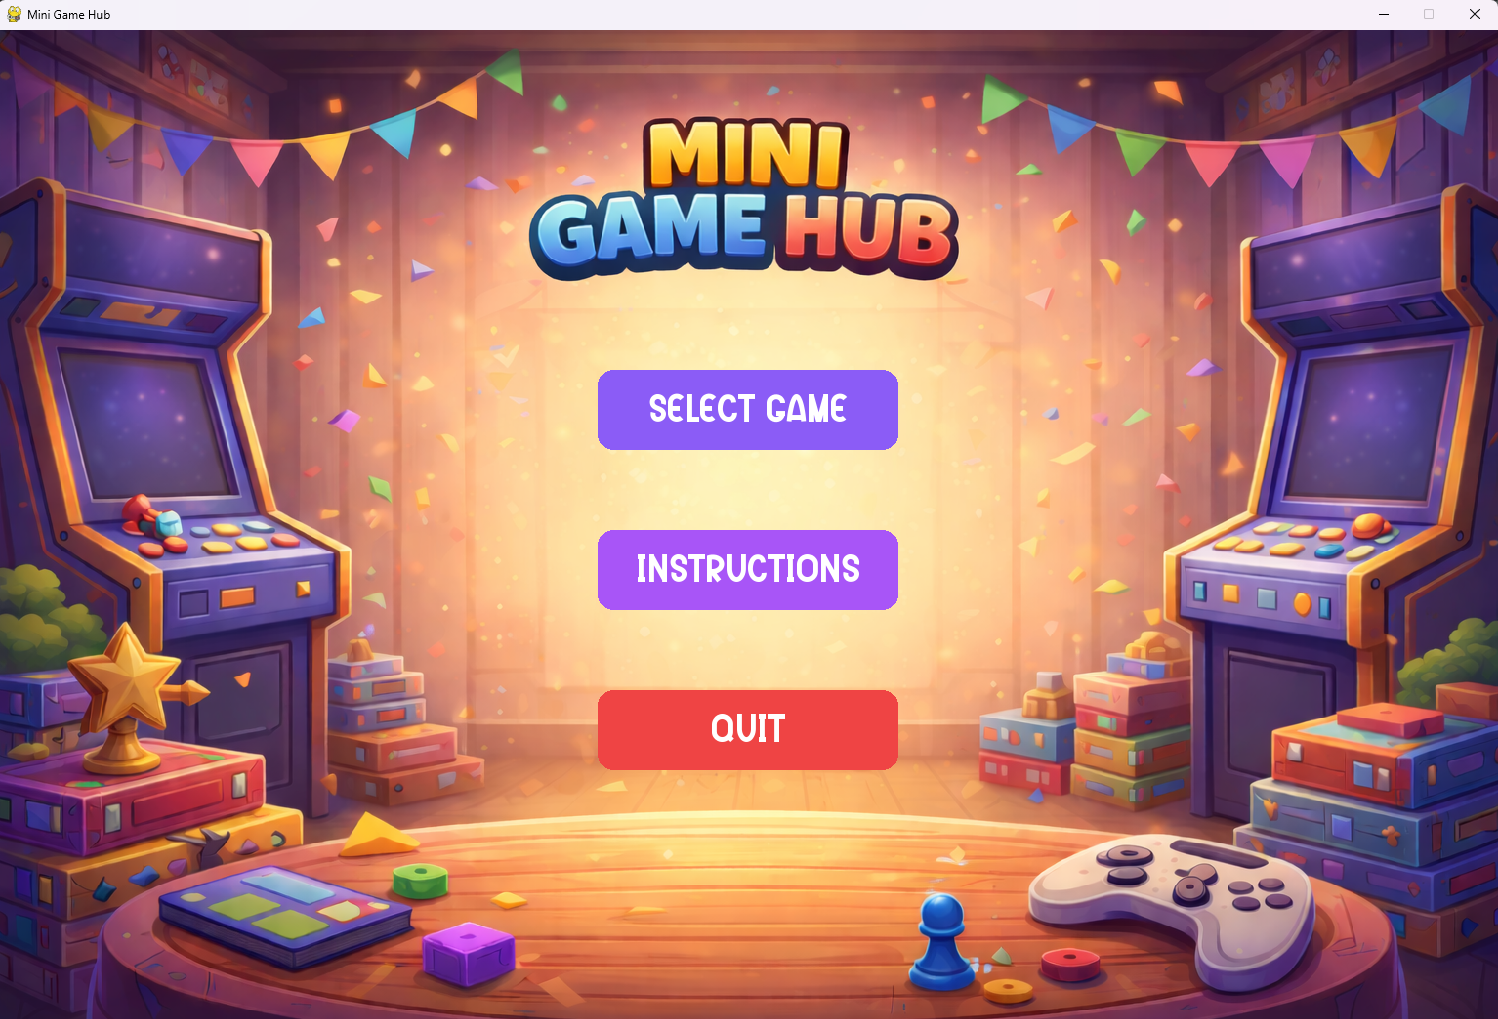
\includegraphics[width=0.45\textwidth]{PyGame1}
    \caption{PyGame1}
    \label{fig:PyGame1}
\end{figure}

\begin{figure}[h]
   \centering
    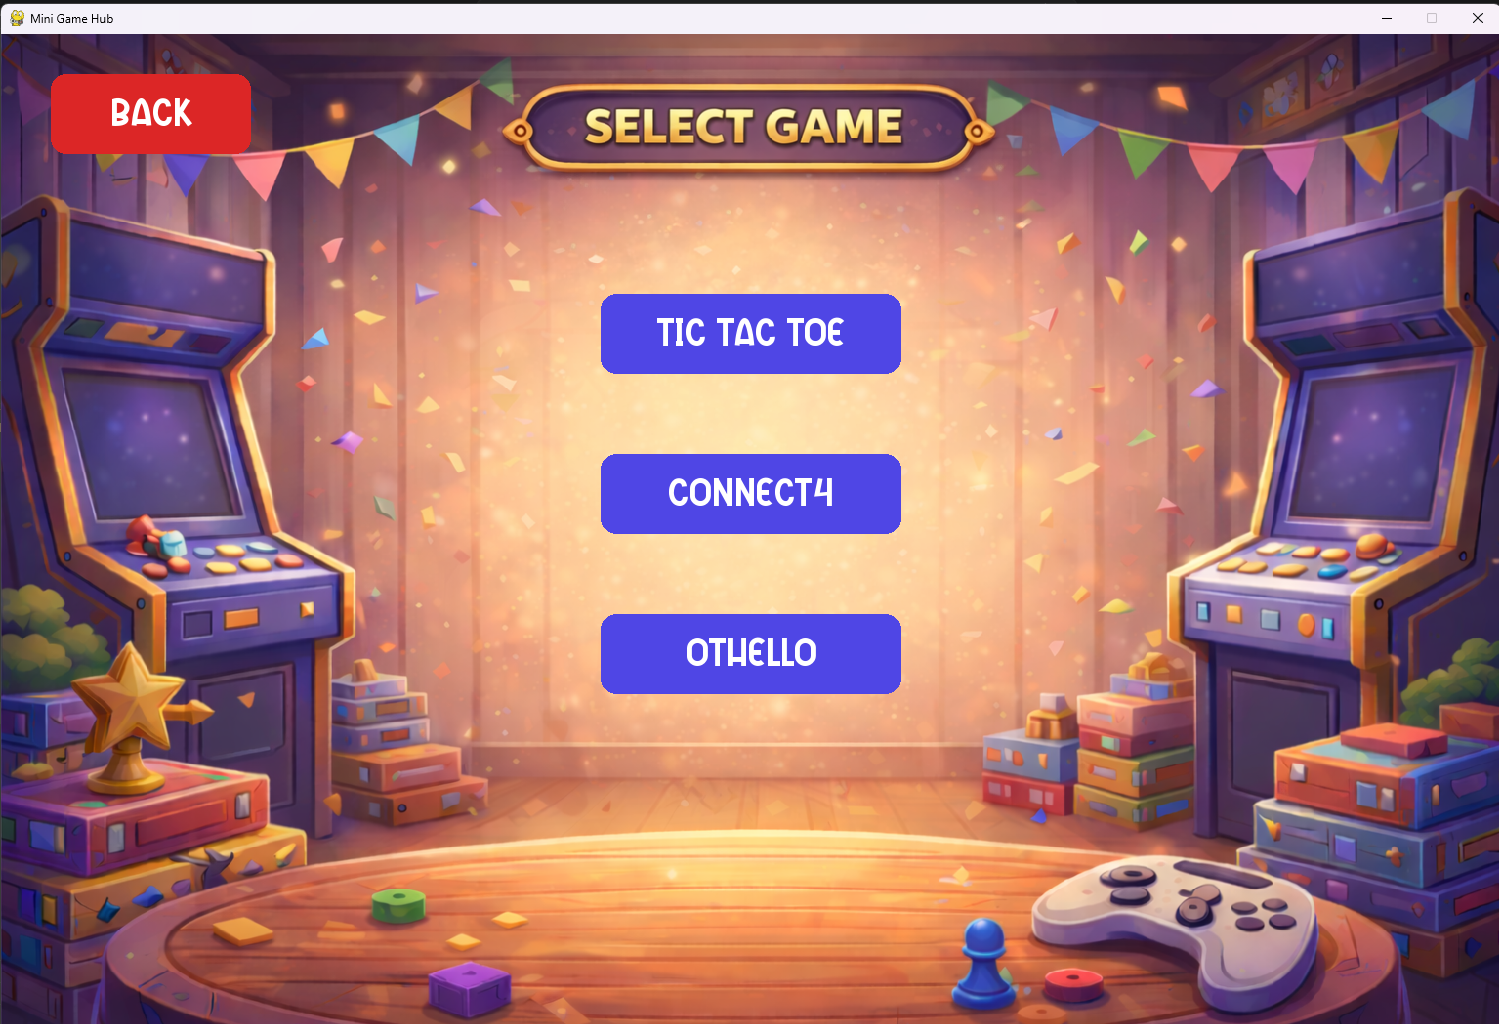
\includegraphics[width=0.45\textwidth]{PyGame2}
    \caption{PyGame2}
    \label{fig:PyGame2}
\end{figure}

\subsection{Playing Games}
After clicking any game button, you will be directed to the respective game boards of TicTacToe, Connect4 or Othello as shown below \ref{fig:tictactoe} \ref{fig:connect4} \ref{fig:othello}.
In each game, the turn's of players are shown on the top of the board and points are displayed for Othello game (beside game board).
Different previews and symbols(like different colors or symbols) are also shown for each player.

\begin{figure}[h]
    \centering
    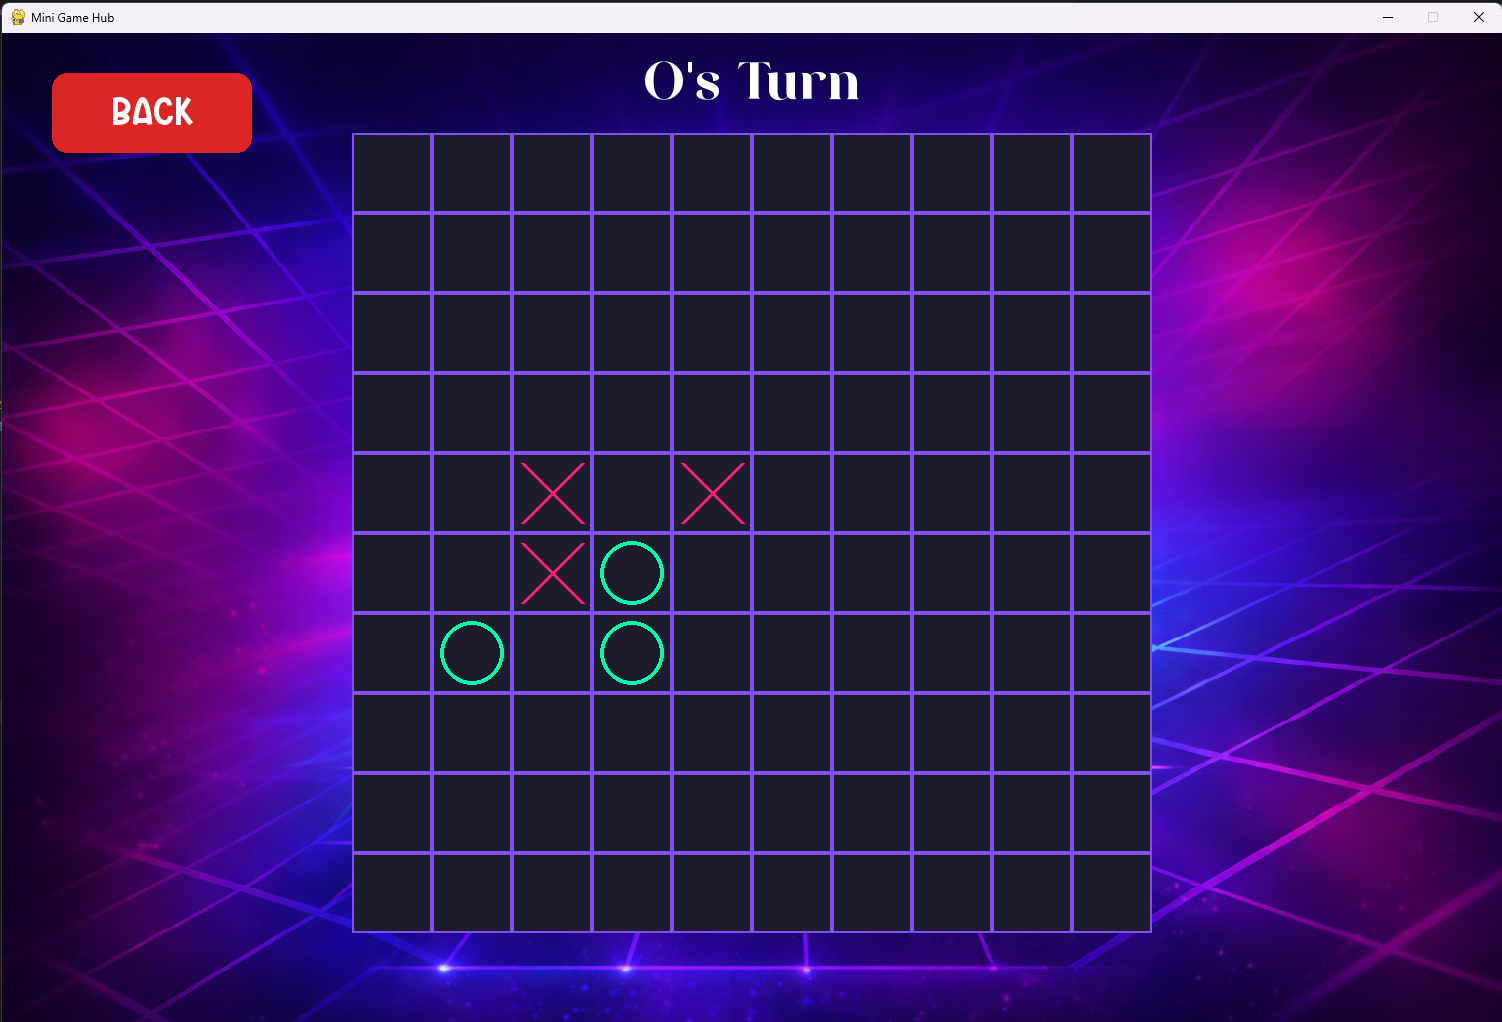
\includegraphics[width=0.75\textwidth]{tictactoe}
    \caption{tictactoe}
    \label{fig:tictactoe}
\end{figure}

\begin{figure}[h]
    \centering
    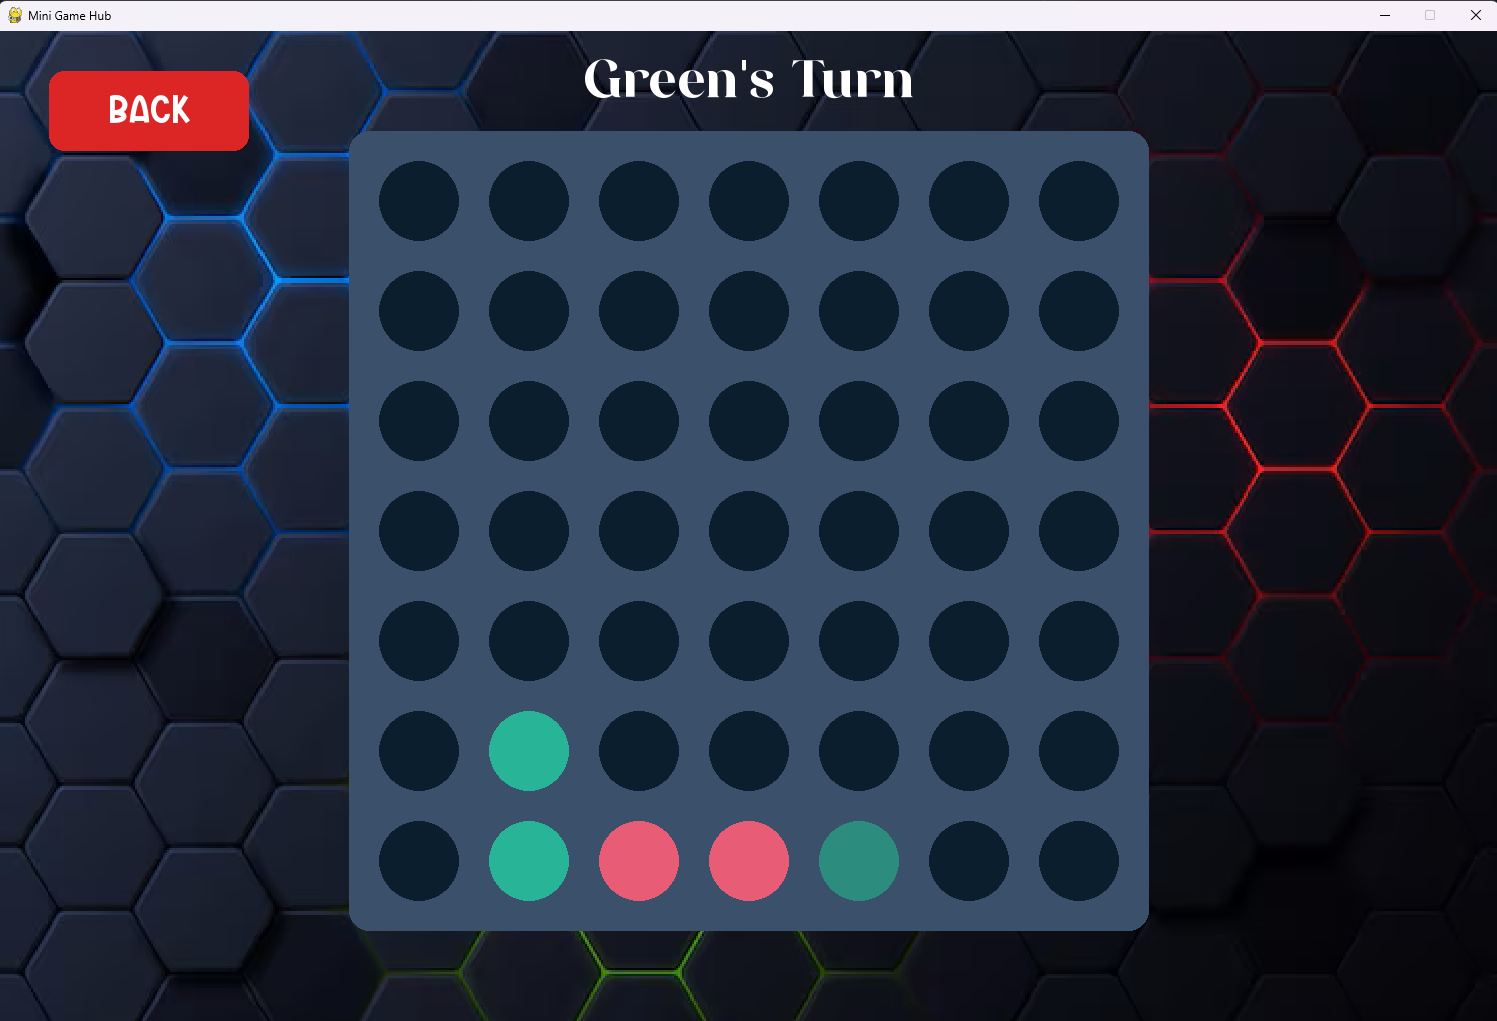
\includegraphics[width=0.75\textwidth]{connect4}
    \caption{connect4}
    \label{fig:connect4}
\end{figure}

\begin{figure}[h]
    \centering
    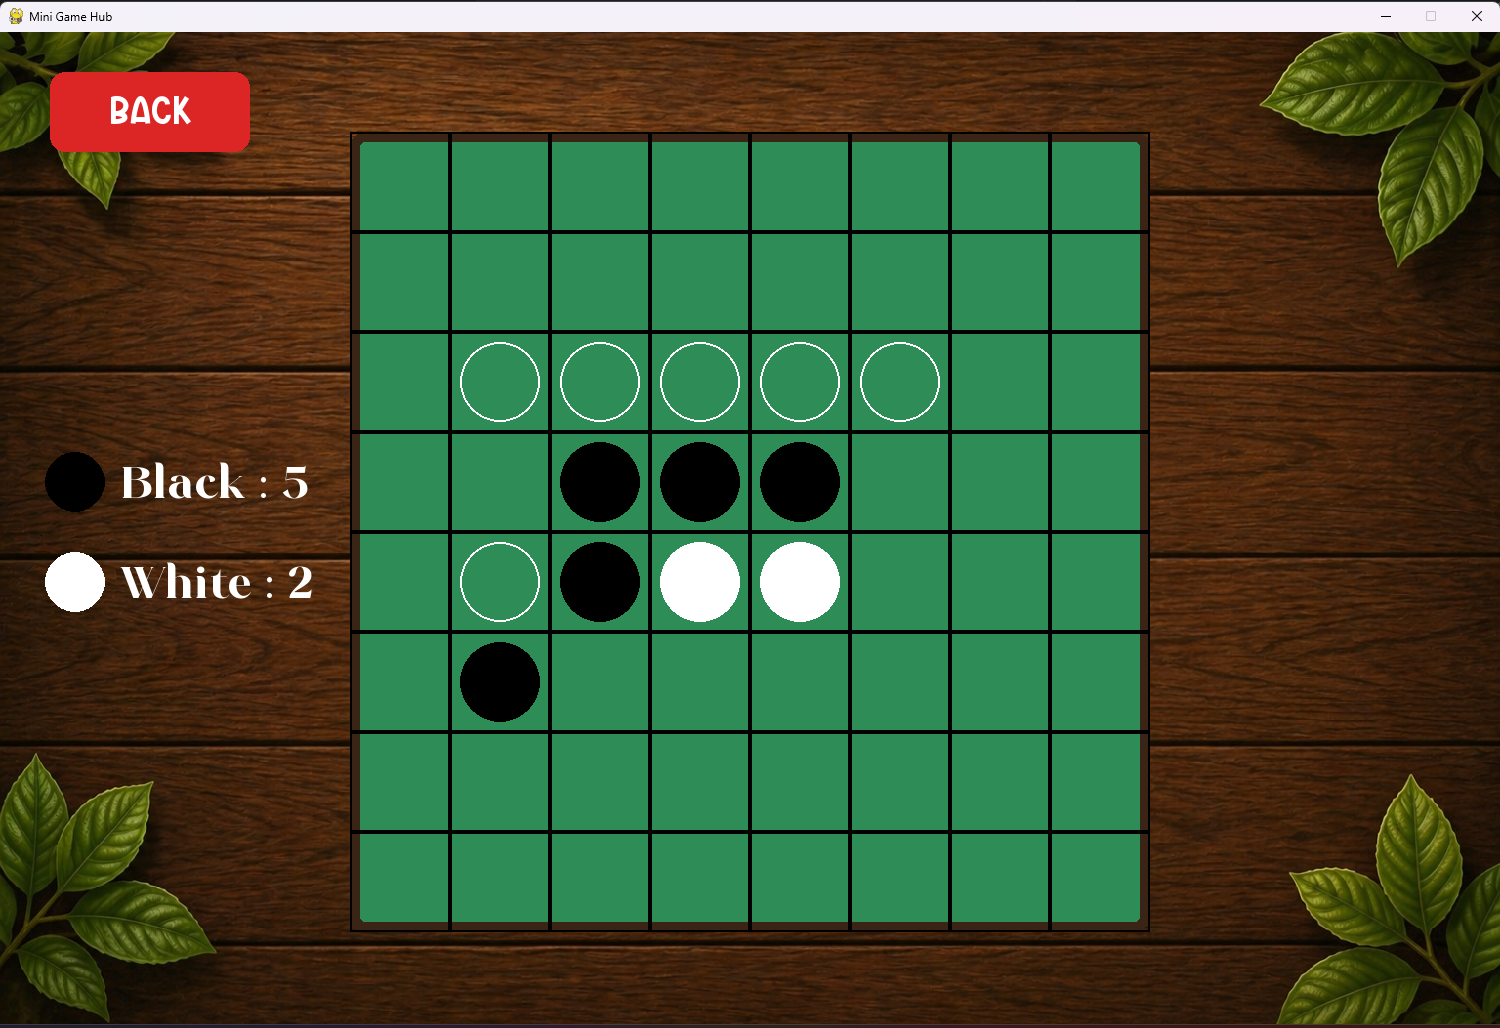
\includegraphics[width=0.75\textwidth]{othello}
    \caption{othello}
    \label{fig:othello}
\end{figure}

\subsection{Leaderboard and Matplotlib options}
After the game ends, you will be redirect to a page which has "Show leaderboard by wins or losses or wins/loss ratio", "Show matplotlib charts", "Play again" or "QUIT" Buttons.
You can see whatever you want by clicking on the buttons you wish. The window is shown here \ref{fig:PyGame3}

\begin{figure}[h]
    \centering
    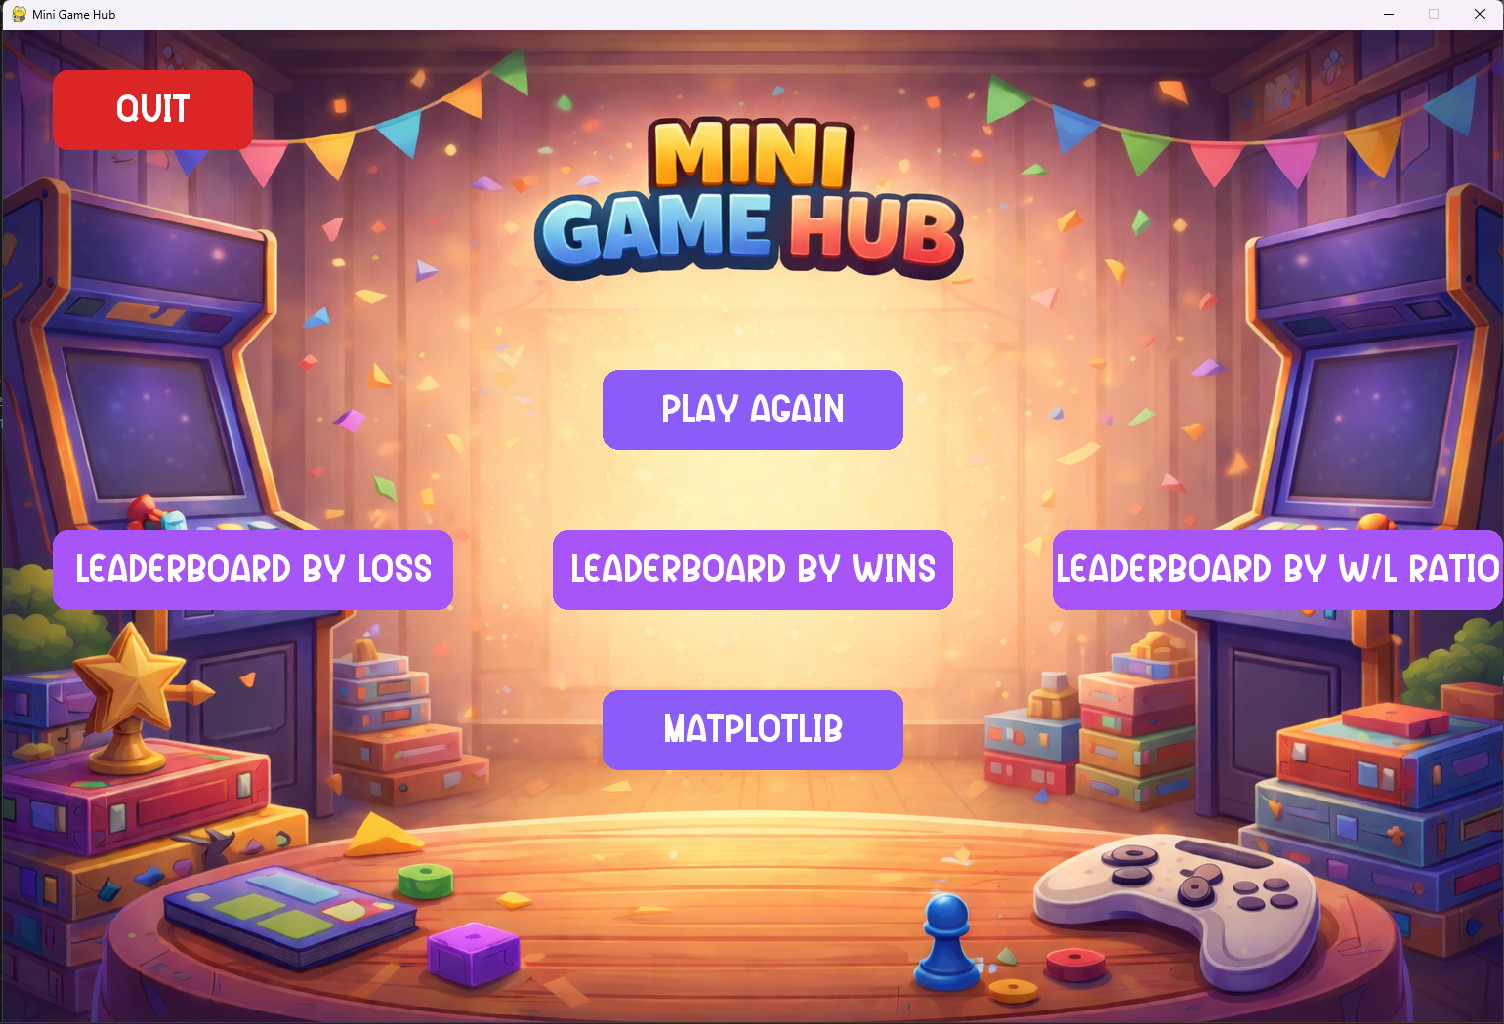
\includegraphics[width=0.75\textwidth]{PyGame3}
    \caption{PyGame3}
    \label{fig:PyGame3}
\end{figure}

\section{Challenges faced and Future Implementations}
There are many challenges that we faced during this project.

\begin{itemize}
    \item Scaling difference in Windows and Linux which was unnoticed in the beginning but when we ran in wsl terminal, we got to know about it. We overcame it by changing display ratio in Windows.
    \item At starting, main.sh was not running in Windows. We overcame it by .gitattributes
    \item Leaderboard was not printing properly due to trailing spaces . We overcame it by command \texttt{tr -d "}
    \item Display board was not updating properly as expected due to many for loops. We overcame it by implementing handle click method in every game.
\end{itemize}

Future Implementations:

\begin{itemize}
    \item Adding Instructions page after clicking Instructions button in main menu.
    \item Adding background music.
    \item Reset passsword functionality in User Authentication.
    \item Adding more matplotlib charts.
\end{itemize}

\section{References}
\begin{itemize}

\item SHA-256 hashing in Bash: use the sha256sum command
\item Python inheritance: \href{https://docs.python.org/3/tutorial/classes.html}{docs.python.org/3/tutorial/classes.html}
\item Pygame CE official documentation: \href{https://pyga.me}{pyga.me}
\item Rules for the games mentioned:
\begin{enumerate}
    \item \href{https://tttxo.com/}{Tic-tac-toe}
    \item \href{https://www.mathsisfun.com/games/reversi.html}{Othello (reversi)}
    \item \href{https://www.mathsisfun.com/games/connect4.html}{Connect4}
\end{enumerate}

\end{itemize}
\end{document} 